\documentclass{article}

\usepackage{fancyhdr}
\usepackage{extramarks}
\usepackage{amsmath}
\usepackage{amsthm}
\usepackage{amsfonts}
\usepackage{tikz}
\usepackage[plain]{algorithm}
\usepackage{algpseudocode}
\usepackage{enumerate}
\usepackage{amssymb}

\usetikzlibrary{automata,positioning}

%
% Basic Document Settings
%

\topmargin=-0.45in
\evensidemargin=0in
\oddsidemargin=0in
\textwidth=6.5in
\textheight=9.0in
\headsep=0.25in

\linespread{1.1}

\pagestyle{fancy}
\lhead{\hmwkAuthorName}
\chead{\hmwkClass\ (\hmwkClassInstructor\ \hmwkClassTime): \hmwkTitle}
\rhead{\firstxmark}
\lfoot{\lastxmark}
\cfoot{\thepage}

\renewcommand\headrulewidth{0.4pt}
\renewcommand\footrulewidth{0.4pt}

\setlength\parindent{0pt}

%
% Create Problem Sections
%

\newcommand{\enterProblemHeader}[1]{
    \nobreak\extramarks{}{Problem \arabic{#1} continued on next page\ldots}\nobreak{}
    \nobreak\extramarks{Problem \arabic{#1} (continued)}{Problem \arabic{#1} continued on next page\ldots}\nobreak{}
}

\newcommand{\exitProblemHeader}[1]{
    \nobreak\extramarks{Problem \arabic{#1} (continued)}{Problem \arabic{#1} continued on next page\ldots}\nobreak{}
    \stepcounter{#1}
    \nobreak\extramarks{Problem \arabic{#1}}{}\nobreak{}
}

\setcounter{secnumdepth}{0}
\newcounter{partCounter}
\newcounter{homeworkProblemCounter}
\setcounter{homeworkProblemCounter}{1}
\nobreak\extramarks{Problem \arabic{homeworkProblemCounter}}{}\nobreak{}

%
% Homework Problem Environment
%
% This environment takes an optional argument. When given, it will adjust the
% problem counter. This is useful for when the problems given for your
% assignment aren't sequential. See the last 3 problems of this template for an
% example.
%
\newenvironment{homeworkProblem}[1][-1]{
    \ifnum#1>0
        \setcounter{homeworkProblemCounter}{#1}
    \fi
    \section{Problem \arabic{homeworkProblemCounter}}
    \setcounter{partCounter}{1}
    \enterProblemHeader{homeworkProblemCounter}
}{
    \exitProblemHeader{homeworkProblemCounter}
}

%
% Homework Details
%   - Title
%   - Due date
%   - Class
%   - Section/Time
%   - Instructor
%   - Author
%

\newcommand{\hmwkTitle}{Tutorial 3}
\newcommand{\hmwkDueDate}{February 2, 2021}
\newcommand{\hmwkClass}{CZ2003}
\newcommand{\hmwkClassTime}{SS3}
\newcommand{\hmwkClassInstructor}{Assoc Prof Alexei Sourin}
\newcommand{\hmwkAuthorName}{\textbf{Pang Yu Shao}}
\newcommand{\hmwkAuthorID}{\textbf{U1721680D}}

%
% Title Page
%

\title{
    \vspace{2in}
    \textmd{\textbf{\hmwkClass:\ \hmwkTitle}}\\
    \normalsize\vspace{0.1in}\small{Due\ on\ \hmwkDueDate\ at 10:30am}\\
    \vspace{0.1in}\large{\textit{\hmwkClassInstructor\ - \hmwkClassTime}}
    \vspace{3in}\\
    \hmwkAuthorName\\
    \hmwkAuthorID
}

\date{01/02/2021}

\renewcommand{\part}[1]{\textbf{\large Part \Alph{partCounter}}\stepcounter{partCounter}\\}

%
% Various Helper Commands
%

% Useful for algorithms
\newcommand{\alg}[1]{\textsc{\bfseries \footnotesize #1}}

% For derivatives
\newcommand{\deriv}[1]{\frac{\mathrm{d}}{\mathrm{d}x} (#1)}

% For partial derivatives
\newcommand{\pderiv}[2]{\frac{\partial}{\partial #1} (#2)}

% Integral dx
\newcommand{\dx}{\mathrm{d}x}

% Alias for the Solution section header
\newcommand{\solution}{\textbf{\large Solution}}

% Probability commands: Expectation, Variance, Covariance, Bias
\newcommand{\E}{\mathrm{E}}
\newcommand{\Var}{\mathrm{Var}}
\newcommand{\Cov}{\mathrm{Cov}}
\newcommand{\Bias}{\mathrm{Bias}}

\begin{document}

\maketitle

\pagebreak

\begin{homeworkProblem}
    Write parametric formulas \(x(u)\), \(y(u)\) for the ray cast from the point with
    coordinates (1, 2) through the point with coordinates (4, 3). Define the domain
    for the parameter \(u\).\\

    \textbf{Solution}\\
    \(x(u) = x1 + u(x2 - x1)\)\\
    \(x(u) = 1 + u(4 - 1)\)\\
    \(\mathbf{x(u) = 1 + 3u}\)\\\\
    \(y(u) = y1 + u(y2 - y1)\)\\
    \(y(u) = 2 + u(3 - 2)\)\\
    \(\mathbf{y(u) = 2 + u}\)\\\\

    For Rays, Domain: \(u \in [0, \inf)\)
    

\end{homeworkProblem}

\begin{homeworkProblem}
    \textbf{Using an equation in intercepts}, obtain an \textbf{implicit} formula 
    \(f(x,y)=0\) for the straight line intersecting the coordinate axes X and 
    Y at the points with coordinates (-2, 0) and (0, 3), respectively.\\

    \textbf{Solution}\\
    Intercept form: \\
    \(\frac{x}{a} + \frac{y}{b} = 1\), where\\
    \(a = -2, y = 3\)\\\\
    \(\therefore \mathbf{f(x,y) = \frac{x}{2} - \frac{y}{3} + 1 = 0}\)
    
\end{homeworkProblem}
\pagebreak
\begin{homeworkProblem}
    With reference to Figure Q3, write parametric functions \(x(u)\), \(y(u)\), 
    \(u\in[0, 1]\)
    defining this spiral curve which has to be drawn clockwise from the point with
    coordinates \((0, 0.3)\). \\

    \begin{figure}[H]
        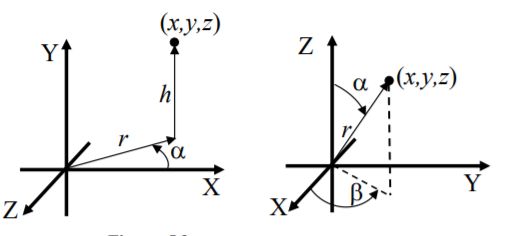
\includegraphics[width=6cm]{fig/q3.PNG}
        \centering
    \end{figure}

    \textbf{Solution}\\
    Flip x and y from notes examples, such that x = sin, y = cos.\\
    Since 2 spirals, argument of sin/cos functions will be \(4\pi u\)

    \(\mathbf{ x(u) = (0.3 + 1.2u)cos(-4\pi u + \pi / 2) }\)\\
    \(\mathbf{ y(u) = (0.3 + 1.2u)sin(-4\pi u + \pi / 2) }\)

    


\end{homeworkProblem}
\pagebreak
\begin{homeworkProblem}
    Based on the way how polar coordinates are mapped to Cartesian, propose
    parametric functions \(x(u)\), \(y(u)\), \(u \in [0, 1]\) which make the trigonometric
    sinusoidal curve (sine wave) follow a semicircle
    (half circle) with the radius of 0.75. The curve has to make 10 periodic
    oscillations (cycles) moving counterclockwise around the semicircle with the
    oscillations amplitude of ±0.25 as shown in Figure Q4.\\
    \begin{figure}[H]
        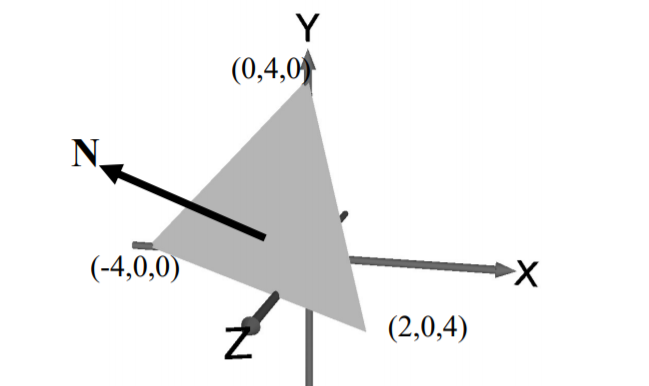
\includegraphics[width=14cm]{fig/q4.PNG}
        \centering
    \end{figure}
    \textbf{Solution}\\
    10 oscilations -- argument of sine wave function: \(20\pi u\)\\
    Amplitude of sine wave: 0.25 (0.75 +- 0.25)\\
    
    
    \(r = 0.75 + 0.25sin(20\pi u)\)\\
    \(x = rcos(u)\)\\
    \(\mathbf{x = cos(\pi u) (0.75 + 0.25sin(20\pi u))}\)\\\\
    \(y = rsin(u)\)\\
    \(\mathbf{y = sin(\pi u) (0.75 + 0.25sin(20\pi u))}\)\\
    \(\mathbf{u \in [0,1]}\)\\

    \begin{figure}[H]
        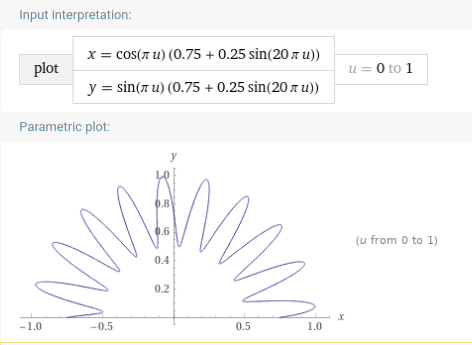
\includegraphics[width=10cm]{fig/q4ans.PNG}
        \centering
    \end{figure}

\end{homeworkProblem}

    



\end{document}